% Supplementary Information — Digital lifestyles and consumption-based carbon emissions
\documentclass[11pt,a4paper]{article}
\usepackage[utf8]{inputenc}
\usepackage[T1]{fontenc}
\usepackage[english]{babel}
\usepackage[margin=2.5cm]{geometry}
\usepackage{booktabs}
\usepackage{graphicx}
\usepackage{xcolor}
\usepackage[hidelinks]{hyperref}
\graphicspath{{../output/}}
\newcommand{\todo}[1]{\textcolor{red}{[TODO: #1]}}
\renewcommand{\thesection}{S\arabic{section}}
\renewcommand{\thetable}{S\arabic{table}}
\renewcommand{\thefigure}{S\arabic{figure}}

\title{Supplementary Information:\\
Digital lifestyles and consumption-based carbon emissions}
\author{David Andersson \and Mathias Lehner \and Mikael Eriksson}
\date{Draft --- \today}

\begin{document}
\maketitle

\section{Sample population and external validity}

\subsection{Recruitment frames and eligibility}
Participants were recruited in spring 2024 through Sweden's national digital
mailbox service (\emph{Mina meddelanden}). The sampling frame comprised two
invitation streams. The random frame contained approximately 80,000 adults in
single-adult households, with children up to age 14 permitted, drawn from
Statistics Sweden population registers among people connected to a digital
mailbox. A separate non-random frame contained approximately 100,000 adults
from electoral districts in which the Green Party received a substantially
higher vote share than the national average. Eligibility required a smartphone
with electronic identification (BankID), bank-account linkage through a secure
interface, and consent to survey participation and registry linkage.

Unlike analyses designed to estimate population means from the random frame,
the present associational analysis currently pools participants from both
streams. This increases precision but means that the unweighted analytical
sample is not nationally representative. The target population is further
restricted by design to adults in single-adult households connected to a
digital mailbox and by participation requirements involving a smartphone and
bank-account linkage.

\subsection{Sample construction}
Table~\ref{tab:sample-flow} reports the stages currently available from the
digital-lifestyles pipeline. A valid transaction month has more than SEK 3,000
in non-excluded spending, and at least three such months are required within
the year preceding the baseline survey. The large reduction between the survey
and transaction stages reflects bank linkage and transaction-coverage
requirements, not item nonresponse alone.

\begin{table}[htbp]
	\centering
	\caption{Sample flow for the pooled recruitment streams.}
	\label{tab:sample-flow}
	\begin{tabular}{@{}lr@{}}
		\toprule
		Stage & Remaining \\
		\midrule
		Invited, random frame & $\approx80,000$ \\
		Invited, green-area oversample & $\approx100,000$ \\
		Baseline survey & 12,153 \\
		At least 8 of 11 composite items answered & 11,172 \\
		At least three valid transaction months & 4,392 \\
		Register and profile controls linked & 4,251 \\
		Complete main analysis sample & 4,250 \\
		\bottomrule
	\end{tabular}
	\begin{flushleft}\footnotesize
		Note: The invitation counts describe the recruitment frames and should not
		be interpreted as response denominators until duplicate invitations and the
		current TRE linkage snapshot have been reconciled by recruitment stream.
	\end{flushleft}
\end{table}

\subsection{Representativeness and reliability analyses}
The next TRE run will report four complementary checks. First, recruitment
counts will be tabulated separately for the random and green-area streams at
the invitation, survey, battery, transaction, control-linkage, and analytical
stages. Second, the analytical subset from the
random frame will be compared with the invited random frame on age, gender,
and major-city residence. These comparisons describe observed selection into
the linked analytical sample; they cannot assess selection on unobserved
characteristics.

Third, the fully adjusted spending and emissions gradients will be estimated
separately in the random-frame and green-area samples. Agreement in direction
and magnitude would show that the pooled result is not generated solely by the
non-random oversample. Fourth, inverse-probability weights for entering the
analysis from the random frame will be estimated from age group, gender, and
major-city residence, trimmed at the 99th percentile, and normalized to mean
one. Weighted random-frame estimates will be compared with the unweighted
pooled and random-frame estimates. Weighting addresses selection on these
observed dimensions only and does not establish national representativeness.

\todo{Insert recruitment-stream flow, random-frame benchmark, sampling-weight
diagnostics including effective sample size, and pooled/stream-specific/weighted
spending and emissions gradients from recruitment\_stream\_flow.csv,
random\_frame\_benchmark.csv, sampling\_ipw\_cell\_balance.csv, and
sampling\_ipw\_diagnostics.csv, and representativeness\_gradients.csv.}

Observed spending also depends on how many accounts each participant connected.
The main estimate is therefore compared with models controlling for account
count, account-count strata, and samples whose observed spending lies within
25--200\% and 50--150\% of register income. These checks assess transaction
coverage rather than recruitment representativeness and are not treated as
validated corrections for missing accounts.

\section{Survey instruments}

\subsection{Baseline digital-practice battery}
The baseline items ask, ``Approximately how often have you used the following
equipment during the past three months?'' (q11) and ``Approximately how often
have you done the following things during the past three months?'' (q11b).
Every item uses the same ordered response options: (1) not used, (2) less often
than weekly, (3) one to six times per week, (4) daily, (5) several times per
day, and (6) several times per hour. Table~\ref{tab:digital-items} gives the
item wording translated from Swedish. The original Swedish questionnaires and
codebooks will be supplied in the study repository.

\begin{table}[htbp]
	\centering
	\caption{Baseline items used to construct the digital-practice composites.}
	\label{tab:digital-items}
	\begin{tabular}{@{}p{0.14\textwidth}p{0.66\textwidth}p{0.08\textwidth}@{}}
		\toprule
		Item & English translation & Revised index \\
		\midrule
		q11\_1 & Desktop or laptop computer & Yes \\
		q11\_2 & Mobile phone or smartphone & Yes \\
		q11\_3 & Television & Yes \\
		q11\_4 & Game console & Yes \\
		q11\_5 & Tablet or e-reader & Yes \\
		q11b\_1 & Watched films, series, or YouTube & Yes \\
		q11b\_2 & Talked on the phone or had video calls & Yes \\
		q11b\_3 & Used social media (e.g., Facebook) & Yes \\
		q11b\_4 & Searched for information online & Yes \\
		q11b\_5 & Played computer or video games & Yes \\
		q11b\_6 & Read books or magazines digitally & Yes \\
		q11b\_7 & Shopped on e-commerce sites & No \\
		q11b\_8 & Sold something (e.g., on an online marketplace) & No \\
		\bottomrule
	\end{tabular}
	\begin{flushleft}\footnotesize
	Note: All 13 items belong to the originally registered index. The revised
	index excludes q11b\_7 and q11b\_8 as a post-registration correction.
	\end{flushleft}
\end{table}

The calls item combines ordinary phone calls and video calls in one response.
It therefore cannot distinguish occupational video meetings from private
communication. Analyses of this item are interpreted as exploratory diagnostics
of a mixed communication measure.

\subsection{Device-assisted mobile screen time}
The endline item asks respondents how much time they spend using their mobile
phone and instructs them to open iOS ``Screen Time'' or Android ``Digital
Wellbeing'' and report the displayed average daily use for the previous week.
Hours and minutes are entered in separate fields. Respondents can instead select
``I have not activated that function'' or ``Skip the question/I cannot find the
information.'' We convert the two fields to decimal hours per day and exclude
values above 18 hours. The survey does not record operating system, and the item
measures mobile-device use rather than total time across all digital devices.

\subsection{Endline activity battery}
The endline battery asks, ``How often during the past 12 months have you done
the following?'' Responses range from (1) never, through (2) once during the
past 12 months, (3) once every six months, (4) once per quarter, (5) once per
month, and (6) once per week, to (7) several times per week.

The out-of-home/social-activity composite contains visiting a library
(F88\_4), attending a sports event (F88\_5), attending a cultural event such as
an art exhibition, theatre performance, or concert (F88\_6), inviting someone
home for dinner (F88\_7), dancing (F88\_8), exercising (F88\_18), and spending
time in nature or outdoor recreation (F88\_21). The at-home composite contains
listening to an audiobook (F88\_11), listening to music (F88\_12), reading a
book (F88\_13), watching a film (F88\_14), and watching a television series
(F88\_16). The domain labels are analytical groupings: individual activities,
especially exercise and reading, need not occur exclusively inside or outside
the home.


\section{Analysis classification}
\todo{Table classifying every reported analysis as originally registered
(doi:10.17605/OSF.IO/RE7BS), post-registration correction, or exploratory,
with the corresponding output file and specification.}

\section{Additional robustness}
\todo{Account-coverage strata, DeSO fixed effects, nonlinear age adjustment,
alternative index scalings, and the 13-item and no-calls ladders
(stepwise\_table.csv, index\_variants.csv, coverage\_robustness.csv).}

\subsection{Mobile screen time}
Among 2,200 respondents with a usable phone reading, mean mobile screen time was
4.39 hours per day (median 3.95; SD 2.41). The correlation with the digital
lifestyle index was weak among the 2,082 respondents with both measures
($r=0.134$, $R^2=0.018$). In the fully adjusted complete-case subsample,
measured screen time was not associated with annual emissions ($27$ kg
CO\textsubscript{2}e per hour; 95\% CI: $-10$ to $64$; $p=0.148$). When both
measures were standardized and entered jointly, the index remained associated
with emissions ($233$ kg per SD; 95\% CI: $138$--$329$), whereas mobile screen
time did not ($29$ kg per SD; 95\% CI: $-59$ to $117$).

\subsection{Reported leisure activities}
\begin{table}[htbp]
	\centering
	\caption{Change in the digital-practice gradient after adjustment for
		reported leisure activities ($N=2,392$).}
	\begin{tabular}{@{}llrrr@{}}
		\toprule
		Outcome & Additional adjustment & kg CO\textsubscript{2}e/SD & 95\% CI & Attenuation \\
		\midrule
		Transport & None & 62.7 & 10.4--115.1 & 0.0\% \\
		Transport & Out-of-home/social & 61.6 & 9.3--113.9 & 1.8\% \\
		Transport & Both composites & 56.7 & 4.4--109.0 & 9.6\% \\
		Total emissions & None & 237.8 & 147.9--327.7 & 0.0\% \\
		Total emissions & Out-of-home/social & 227.4 & 137.9--316.9 & 4.4\% \\
		Total emissions & Both composites & 213.2 & 123.1--303.2 & 10.3\% \\
		\bottomrule
	\end{tabular}
\end{table}

\subsection{Heterogeneity}
Adjusted subgroup estimates were $150$, $263$, $232$, and $561$ kg per SD for
ages 18--29, 30--44, 45--64, and 65+, respectively. The oldest-group estimate
was imprecise (95\% CI: $-544$ to $1,665$). Interactions were not statistically
significant for gender ($p=0.134$) or major-city residence ($p=0.323$).
\todo{Add the formal joint age-group interaction test.}

\begin{figure}[htbp]
	\centering
	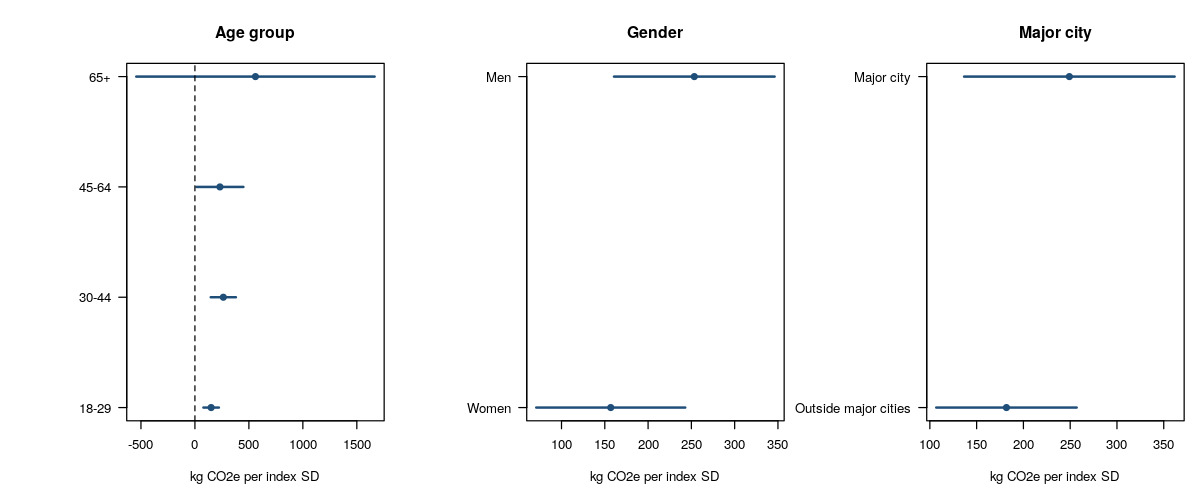
\includegraphics[width=\textwidth]{2026-10-13/het_plot.png}
	\caption{Fully adjusted digital-practice gradients by age group, gender, and
		major-city residence. Points show subgroup coefficients and HC3 95\%
		confidence intervals.}
\end{figure}

\end{document}
